\documentclass{report}

\author{Nikhil Verma}
\usepackage{tikz}
\usepackage{caption}
% \usetikzlibrary{shapes,arrows,positioning}
\usetikzlibrary{automata,arrows,positioning,calc}


\begin{document}
\begin{figure}
	\centering
	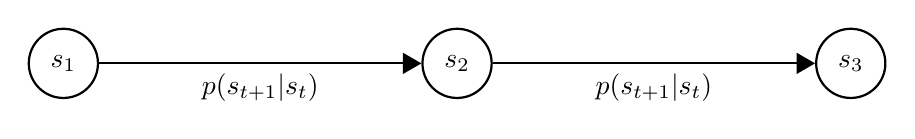
\begin{tikzpicture}[->, >=triangle 60, auto, thick, node distance=5cm]
		\tikzstyle{every state}=[fill=white,draw=black,thick,text=black,scale=1]
		\node[state]    (A)               {$s_1$};
		\node[state]    (B)[right of=A]   {$s_2$};
		\node[state]    (C)[right of=B]   {$s_3$};
		\path
		(A) edge[below] node{$p(s_{t+1}|s_t)$} (B)
		(B) edge[below] node{$p(s_{t+1}|s_t)$} (C);
	\end{tikzpicture}
	\caption*{A Markov Chain}

	\vspace{1cm}

	\centering
	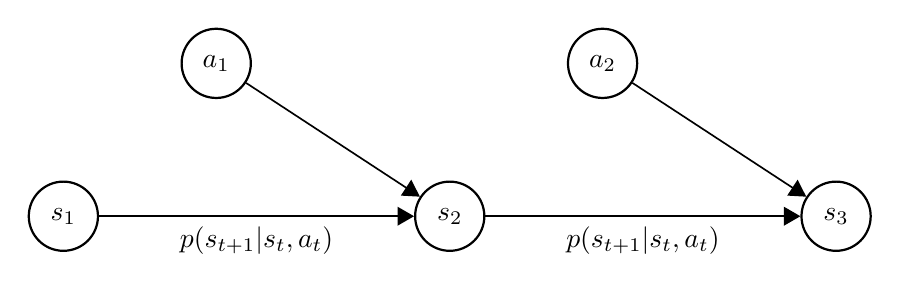
\begin{tikzpicture}[->, >=triangle 60, auto, semithick, node distance=4cm]
		\tikzstyle{every state}=[fill=white,draw=black,thick,text=black,scale=1]
		\node[state]    (A)                 {$s_1$};
		\node[state]    (B)[right = of A]   {$s_2$};
		\node[state]    (C)[right = of B]   {$s_3$};
		\node[state]    (D)[above right = 1.3cm and 1.3cm of A]   {$a_1$};
		\node[state]    (E)[above right = 1.3cm and 1.3cm of B]   {$a_2$};
		\path
		(A) edge[below] node{$p(s_{t+1}|s_t, a_t)$} (B)
		(B) edge[below] node{$p(s_{t+1}|s_t, a_t)$} (C)
		(D) edge[below] (B)
		(E) edge[below] (C);
	\end{tikzpicture}
	\caption*{A Markov Decision Process (MDP)}

	\vspace{1.5cm}

	\centering
	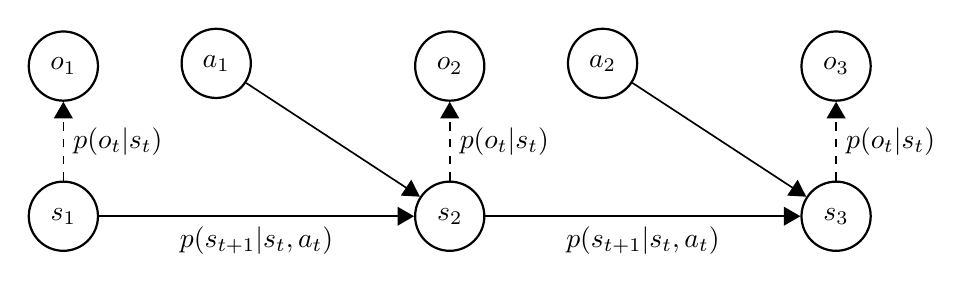
\begin{tikzpicture}[->, >=triangle 60, auto, semithick, node distance=4cm]
		\tikzstyle{every state}=[fill=white,draw=black,thick,text=black,scale=1]
		\node[state]    (A)                 {$s_1$};
		\node[state]    (B)[right = of A]   {$s_2$};
		\node[state]    (C)[right = of B]   {$s_3$};
		\node[state]    (D)[above right = 1.3cm and 1.3cm of A]   {$a_1$};
		\node[state]    (E)[above right = 1.3cm and 1.3cm of B]   {$a_2$};
		\node[state]    (F)[above = 1cm of A]   {$o_1$};
		\node[state]    (G)[above = 1cm of B]   {$o_2$};
		\node[state]    (H)[above = 1cm of C]   {$o_3$};
		\path
		(A) edge[below] node{$p(s_{t+1}|s_t, a_t)$} (B)
		(B) edge[below] node{$p(s_{t+1}|s_t, a_t)$} (C)
		(D) edge[below] (B)
		(E) edge[below] (C);
        \path[dashed]
		(A) edge[right] node{$p(o_t|s_t)$} (F)
        (B) edge[right] node{$p(o_t|s_t)$} (G)
        (C) edge[right] node{$p(o_t|s_t)$} (H);
	\end{tikzpicture}
	\caption*{A Partially Observed Markov Decision Process (POMDP)}
\end{figure}
\end{document}